\chapter{Introduction}

Chemistry involves the study of molecules and materials constructed from nuclei and electrons.
The theoretical description of a chemical system requires a consideration of the size of the system and of the target properties.
An ideal computational chemistry theoretical model would reproduce experimental observables in a computationally tractable amount of time.
In the following sections, Nonvalence anions and the related nonvalence positronic bound states are introduced along with the target properties of interest followed by a discussion of the computational chemistry methods used to describe these systems.

%%%%%%%%%%%%%%%%%%%%%%%%%%%%%%%%%%%%%%%%%%%%%%%%%%%%%%%%%%%%%%%%%%%%%%%%%%%%%%%%%%%%%%%%%%%%%%%%%%%
\section{Chemical Systems}
%%%%%%%%%%%%%%%%%%%%%%%%%%%%%%%%%%%%%%%%%%%%%%%%%%%%%%%%%%%%%%%%%%%%%%%%%%%%%%%%%%%%%%%%%%%%%%%%%%%
% Nonvalence Anions
\subsection{Nonvalence Anions}

Nonvalence anions are formed when a molecule weakly captures an electron in an extremely diffuse orbital.
It is helpful to further differentiate nonvalence anions due to the dominant mechanism of binding into nonvalence electrostatically bound anions (NVEBs) and nonvalence correlation bound anions (NVCBs).
Nonvalence electrostatically bound anions bind an electron using a permanent electrostatic moment.
For example, an electron can be captured by a molecule or molecular cluster with a sufficiently strong dipole moment, creating a nonvalence electrostatically bound anion also called a dipole bound anion (DBA).
Nonvalence correlation bound anions require electron correlation effects to account for the binding of the electron.
This is not to say that the neutral system giving rise to a NVCB lacks any permanent electric moments, but rather, that the uncorrelated description of a system containing these permanent moments will not bind the electron.
%The discussion below includes a more detailed description of these systems along with paradigmatic examples.

\subsubsection{Nonvalence Electrostatically Bound Anions}

Dipole-bound anions (DBAs) are formed when a molecule with sufficiently large dipole moments (1.625 D in the Born-Oppenheimer approximation) capture an electron in a diffuse, nonvalence orbital.\cite{Jordan_Luken_JCP_1976,Gutowski_Jordan_PRA_1996,Barnett_JCP_1988,Fermi_Teller_PhysRev_1947,Turner_Anderson_PhysRev_1968,Crawford_ProcPhysSoc_1967,Garrett_CPL_1970,Garrett_PRA_1971,Lykke_PRL_1984,Desfrancois_Schermann_PRL_1994,Simons_JPCA_2008,Jordan_Wang_Ann_Rev_2003}.
Initially, one may be tempted to think that electron correlation would not play a significant role in such systems given the diffuse nature of the excess electron.
However the excess electron is bound far from the valence electrons, there is a dispersion interaction between the excess electron and the neutral molecule.\cite{Gutowski97,Gutowski98}
However, considering the simplified expression for London dispersion it can be seen that the dispersion interaction is dependent on the polarizability of the two interacting entities.\cite{London1937}
\begin{equation}
	E_{\mathrm{Disp}} = -\left(\frac{3h}{2R^6}\right) \left(\alpha_i \alpha_j \right) \left(\frac{\nu_k \nu_j}{\nu_k + \nu_j} \right)
\end{equation}
where $\alpha$ is the static polarizability, $\nu$ is the ionization potential, and $R$ is the separation distance.
The diffuse electron is spread over a large volume, and therefore has a large polarizability leading to a large dispersion interaction.

\begin{figure}{r}
    \centering
	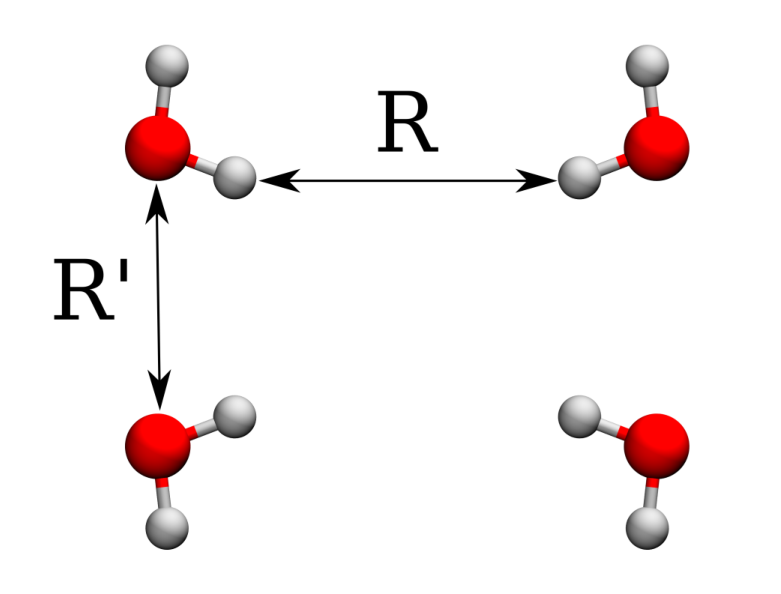
\includegraphics[width=0.9\textwidth,keepaspectratio]{Images/chapter1/h2o4_labeled.eps}
	\caption{A model \ce{(H2O)4} system. The separation between the dimers $R$ is variable, but the separation of two waters within each dimer $r=\SI{2.77514}{\angstrom}$ is fixed.}
	\label{fig:h2o4}
\end{figure}
Nonvalence correlation bound anions are similar to DBAs, but the leading contribution to the binding energy comes from electronic correlation.
Often this means NVCB anions do not posses a dipole moment.
For DBAs, the Hartree-Fock can bind an electron for molecules with dipole moments above the critical threshold, although the electron would be considerably underbound.
For NVCB anions, it has been shown that the HF solution is qualitatively incorrect.
Rather than binding the electron, the HF solution collapses onto the continuum yielding a wavefunction for the neutral plus an excess electron in a continuum orbital.
When this occurs, methods that build upon the HF result such as single reference perturbation theory, or even coupled cluster methods, will also fail to bind the excess electron.
A simple example of this is a model water tetramer cluster that has been studied previously in our group.\cite{Voora2017}
This model system can be seen in fig.~\ref{fig:h2o4}.
This system has no dipole moment, and the electron is bound by electrostatics and correlation effects.
By increasing the separation between the two pairs of water dimers, one can induce a crossover from a nonvalence electrostatically-bound anion to a nonvalence \textit{correlation-bound} anion.
DBAs can serve as a pathway to valence-bound anions\cite{Hendricks_JCP_1998,Compton_JCP_1996,Desfrancois_JCP_1996,Desfrancois_JPCA_1998}, and nonvalence correlation bound anions can as well. \cite{Voora20142}

\begin{figure}{r}
	\centering
	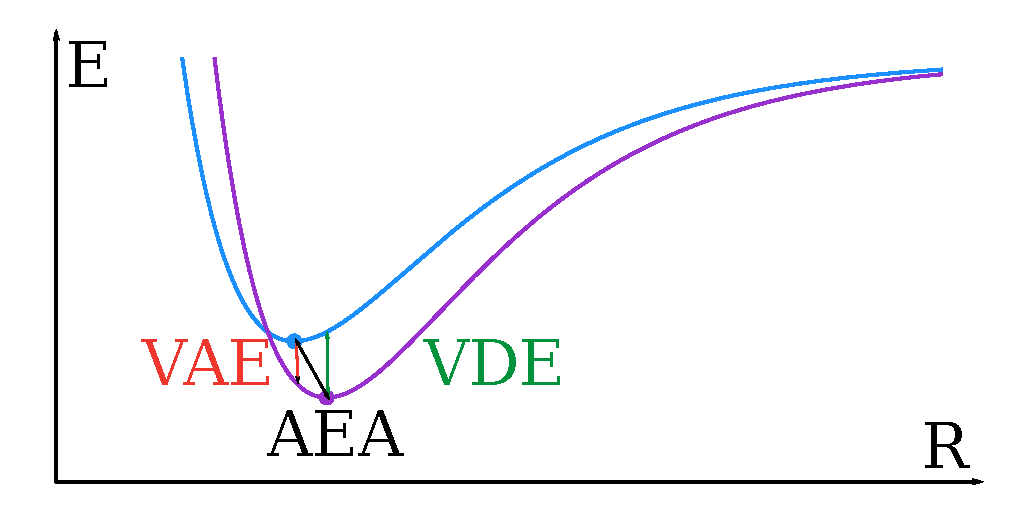
\includegraphics[width=0.9\textwidth,keepaspectratio]{Images/chapter1/morse.eps}
	\caption{Illustrative potential energy curves for a neutral molecule and its corresponding dipole-bound or correlation-bound anion. The energy difference at the neutral geometry is the vertical attachment energy. The energy difference at the anion geometry is the vertical detachment energy. The energy difference between the two respective minima is the \textbf{adiabatic electron affinity}.}
	\label{fig:morse}
\end{figure}

Fig.~\ref{fig:morse} shows illustrative potential energy curves for a hypothetical bound anion.
The coordinate ($R$) represents a collective variable which captures the change in geometry ($\delta R$) that the neutral molecule undergoes upon capturing an electron.
The change in energy associated with binding the electron and the subsequent change in geometry is termed the adiabatic electron affinity.
The change in energy associated only with binding the electron may occur at either the neutral or anionic geometry and is termed the vertical electron affinity and vertical detachment energy respectively.
The extremely diffuse nature of the excess electron in DBAs and NVCB anions often results in a very minor change in geometry.
In the limit of zero change in geometry ($\delta R \rightarrow 0$), the adiabatic electron affinity, vertical electron affinity, vertical detachment energy are equal.
Therefore, for DBAs it is sufficient to calculate only one of these energies.
In practice, and in this work, it is easiest to calculate the vertical electron affinity as this only requires the ground state neutral geometry.
The magnitude by which the electron is bound is also referred to as the electron binding energy (EBE).
The sign convention adopted is that a positive electron binding energy indicates that the the electron is bound.

%%%%%%%%%%%%%%%%%%%%%%%%%%%%%%%%%%%%%%%%%%%%%%%%%%%%%%%%%%%%%%%%%%%%%%%%%%%%%%%%%%%%%%%%%%%%%%%%%%%
% Positron bound states
\subsection{Positron bound states}
Since the theoretical prediction\cite{10.1098/rspa.1928.0023} and subsequent experimental observation\cite{10.1126/science.76.1967.238} of positrons, the exotic antimatter has seen use in a variety of fields such as positron emission tomography in the medical field or in defect characterization in condensed matter physics.\citehere
Modern applications have also included the formation of antihydrogen as a test of fundamental physics regarding violations of charge, parity, and time-reversal symmetries.\citehere

In chemistry, one is interested in the behavior of matter.
It may seem that the study of antimatter is of little interest to chemistry, however through electron-positron interactions serve as an experimental probe to understand the electronic and vibronic structure of molecules.

In order to understand how positrons yield insight into the behavior of molecules, it helps to consider the interaction of a low energy positron with an idealized molecule.
The simplest picture of this process would imply that the positron and electron annihilation rate would be proportional to the number of electrons present.\citehere %surko rev mod
Interestingly, the observed rate of annihilation is orders of magnitude greater for most molecules.\citehere %surko rev mod
The major causes of this increased annihilation rate is the formation of positron-molecule bound states and positron-molecule temporary states (vibrational Feschbach resonances).\citehere
Since the processes are molecule dependent, the experimental characterization of positron annihilation allows one to characterize different molecules.
This also explains the motivation to computationally study positron bound states.
The diffuse positronic states are diffuse analogues to nonvalence anions with direct connection to experiment.

%%%%%%%%%%%%%%%%%%%%%%%%%%%%%%%%%%%%%%%%%%%%%%%%%%%%%%%%%%%%%%%%%%%%%%%%%%%%%%%%%%%%%%%%%%%%%%%%%%%

\section{Theoretical Methods}
%%%%%%%%%%%%%%%%%%%%%%%%%%%%%%%%%%%%%%%%%%%%%%%%%%%%%%%%%%%%%%%%%%%%%%%%%%%%%%%%%%%%%%%%%%%%%%%%%%%
% Molecular quantum mechanics
\subsection{Molecular Quantum mechanics}
Computational chemistry has established itself as a tool for the elucidation and predicition of chemical processes.
For a wide variety of problems such as chemical reactivity, molecular structure, and spectroscopic identification, molecular quantum mechanics provides great insight.

\subsubsection{Schrodinger's Equation}
Molecular Quantum Mechanics  involves the solution of a quantum many body problem for a chemical system. Since experimental observables can be represented as quantum mechanical operators, molecular quantum mechanics can both be verified by comparison to experimental results and also provide atomistic insight into experimental results.
The work in this thesis will only include nonrelativistic systems and time independent states so the time-independent Schrodinger equation will be the target equation which we seek to solve,
\begin{equation}
H_{mol} \Psi = E \Psi,
\end{equation}
where
\begin{equation}
H_{mol} = T_{\mathrm{elec}} + T_{\mathrm{nuc}} + V_{\mathrm{elec-elec}} + V_{\mathrm{elec-nuc}} + V_{\mathrm{nuc-nuc}}.
\end{equation}
The nonrelativistic Schrodinger equation contains the sum over the kinetic energy operators for the electrons and nuclei ($T$) and their corresponding pairwise interaction potentials ($V$).
The dimensionality of this problem restricts its solution to simple, few-particle problems such as the hydrogen atom or the hydrogen molecular anion.

\subsubsection{Born-Oppenheimer Approximation}
A common approximation which enables the solution of the Schrodinger equation is the \gls{boa}.
This approximation involves an assumption that the nuclei are fixed and the electrons see the static potential of these nuclei.
A physical rationalization of this approximation relies on the mass difference between electrons and nuclei as the lightest nucleus, a proton, is roughly 1800 times more massive then an electron.
Due to the extreme difference in masses, it can be assumed that any rearrangement of the nuclei results in an instantaneous rearrangement of the electrons.
This approach has several practical advantages.

First, the dimensionality of the problem is greatly reduced.
By fixing the nuclei, the nuclei degrees of freedom are removed from the the problem.
The nuclei's kinetic energy operators are also removed, and the pairwise intereaction between the nuclei becomes a constant energy shift.

Second, the \gls{boa} allows for a logical source for a basis expansion for the electrons.
Consider the hydrogen molecular ion without the introduction of fixed nuclei, the natural basis for the electron is prolate spherical coordinates /Strumian functions.\todo{fix}
Note that the basis functions have explicit dependence on the electron's coordinates and also the nuclei's coordinates
As the number of nuclei and electrons grows this interdependence becomes an immediate barrier to obtaining a solution to the Schrodinger equation.
By making the electronic wave function only have a paraetric depedence on the nuclei's coordinates, we enable the use of atom centered basis functions.
This approximation is therefore central to the popular \gls{lcao} approach.

Third, the \gls{boa} gives us the concepts of a molecule and its associated potential energy surface.
A potential energy surface is a multidimensional scalar function of a molecule in a particular electronic state in which the energy is a function of the nuclear positions of a molecule.
In modern computational chemsitry, it is routine that we consider that we have a molecule and we can optimize the geometry optimization in ground or excited states.
One expects that these geometries and the associated observables correspond to ground or exctied states of chemical systems.
This way of thinking about molecules depends on a decoupling of the nuclei and electron coordinates enabled by the \gls{boa}.

%%%%%%%%%%%%%%%%%%%%%%%%%%%%%%%%%%%%%%%%%%%%%%%%%%%%%%%%%%%%%%%%%%%%%%%%%%%%%%%%%%%%%%%%%%%%%%%%%%%
% Many Body Methods
% Mean Field Methods
\subsection{Mean Field Methods}

%%%%%%%%%%%%%%%%%%%%%%%%%%%%%%%%%%%%%%%%%%%%%%%%%%%%%%%%%%%%%%%%%%%%%%%%%%%%%%%%%%%%%%%%%%%%%%%%%%%
% Correlation Methods
% TODO edit here
\subsection{Correlated Methods}
Once the Hartree-Fock method, has converged a single Slater determinant wave function is obtained.
The description of the wave function captures many of the salient properties of the system.
For example, if we knew the exact nonrelativistic energy for a system, the HF energy accounts for \shiv{99} of the exact energy.\shiv{cite pople}
We define the missing energy as the correlation energy,
\begin{equation}
E_{\mathrm{corr}} = E_{\mathrm{exact}} - E_{\mathrm{HF}},
\end{equation}
since it is the portion of the energy missed due to the use of averaged interactions between electrons.

If the correlation energy per electron were constant, then computational chemistry would be much easier.
For example, if one were calculating the atomization energy of a water molecule,
\begin{equation}
    E_{\mathrm{atom}} = E_{\mathrm{H2O}} - 2 E_{\mathrm{H}} - E_{\mathrm{O}},
\end{equation}
each term would have a constant shift, and the relative energy difference $E_{\mathrm{atom}}$ would be equivalent if calculated with the exact energy or the HF energy.
Unfortunately this is not the case, and thus we aim to capture the correlation energy accurately for a chemical system.

In this thesis 3 main approaches are used to recover electron correlation:
\begin{itemize}
\item \textbf{Density Function Theory}- Since the Hartree-Fock method neglects $e^{-}$ correlation by using an averaged potential, DFT attempts to modify the effection potential to recover correlation energy.
\item \textbf{Wave function based methods}- Build upon a Hartree-Fock wavefunction and reincorporate correlation through methods such as perturbation theory.
\item \textbf{Stochastic methods}- Randomly sample correlated forms of wave functions, which would be difficult or impossible to solve deterministically, to recover correlation.
\end{itemize}

\subsubsection{Density Functional Theory Methods}
\gls{dft} has seen widespread use since it is an economical, albeit approximate, treatment of electron correlation.\cite{10.1103/RevModPhys.87.897, 10.1002/qua.24259}

\gls{dft} in theory is an exact method.
The first Hohenberg-Kohn theorem establishes an exact mapping between the interaction potential and the electron density.\cite{10.1103/PhysRev.136.B864}
The second Hohenberg-Kohn theorem shows that a variational principle for the energy as a functional of the density exists.\cite{10.1103/PhysRev.136.B864}
While these theorems and extensions for finite temperature, magnetic fields, and other generalizations,\cite{10.1103/PhysRev.137.A1441, 10.1103/PhysRevLett.59.2360,10.1073/pnas.76.12.6062} solidify \gls{dft}'s theoretical footing, they do not indicate how one would practically use \gls{dft}.

In practice, the Kohn-Sham equations are used which maps the density-based Schr{\"o}dinger equation problem on to a fictious noninteracting problem with an effective field,
\begin{equation}
(\hat{T} + \hat{V}_{\mathrm{eff}}) \psi(r) = E \psi(r).
\end{equation}
This formulation resembles a \gls{hf} equation where the interaction potential has been replaced by an effective potential.
This allows one to utilize the standard \gls{hf} machinery and incorporate electron correlation at minimal cost.
The form of the effective potential is what is commonly referred to as the \gls{dft} functional.
These functionals are constructed and parameterized as the exact functional is not known.
This means that althought \gls{dft} is an exact theory, in practice it is not \textit{ab initio}.



\subsubsection{Wave Function Based Methods}
\shiv{mp2}
\shiv{cc}
\shiv{excited state equation of motion methods}

\subsubsection{Stochastic Methods}

\subsubsection{Projector quantum Monte Carlo}
This work involves the application of projector \gls{qmc} methods to locate ground state solutions to the imaginary time Schr{\"o}dinger equation.
The Schr{\"o}dinger equation in imaginary time ($\tau\rightarrow it$) shifted by a constant ($E_r$) is given by eq.~\ref{eq:imSE}.
\begin{equation}
\frac{\partial \ket{\Psi}}{\partial \tau} = - (\hat{H} - E_r) \ket{\Psi}
    \label{eq:imSE}
\end{equation}
The formal solution expanded in energy eigenstates is eq. \ref{eq:formsol}.
\begin{equation}
\ket{\Psi(\tau)} = \sum_{i=0}^{\infty} e^{-(\epsilon_i - E_r) \tau} \ket{\phi_i}
    \label{eq:formsol}
\end{equation}
This means any initial state with nonzero ground state overlap converges to the ground state.
The constant $E_r$ is introduced to maintain normalization. 
To illustrate this consider setting $E_r = 0$, all positive energy states would die off exponentially, but all negative energy states would grow exponentially.
The ground state would grow the fastest so in the long time limit it would dominate, but numerically this involves exponential growth.
This is mitigated by introducing the $E_r$, setting it as close to $E_0$ as possible, and periodically updating it.

The ground state obeys the projection equation (eq.~\ref{eq:proj}).
\begin{equation}
\ket{\Psi_0} \propto \lim_{\tau\rightarrow\infty} e^{-\tau (\hat{H} - E_r)} \ket{\Psi_T}
    \label{eq:proj}
\end{equation}
We now introduce a basis $\ket{B}$ with the only constraint that it is complete.
The propagation of a state in imaginary time (multiplying $\ket{B'}$ and inserting a complete basis $\int dB \ket{B}\bra{B} = 1$)
\begin{equation}
\braket{B'|\Psi(\tau)} = \int dB \braket{B'|e^{-(\hat{H}-E_r)\tau}|B}\braket{B|\Psi(0)}
    \label{eqprop}
\end{equation}
The term $\braket{B'|e^{-(\hat{H}-E_r)\tau}|B}$ is the propagator (Green's function), which is unknown. 
The short time approximation to the Green's function (eq.~\ref{eqshorttimeprop}) however can be be constructed by Suzuki-Trotter decomposition of the exponential, which is exact as $\Delta \tau \rightarrow 0$.\cite{10.1090/S0002-9939-1959-0108732-6,10.1007/BF01609348}
\begin{equation}
\begin{aligned}
    \braket{B'|\Psi(\tau)} = \int dB_{n} \cdots dB_{1} dB &\braket{B'|e^{-(\hat{H}-E_r)\Delta\tau}|B_{n}}\\
                                                          &\braket{B_{n}|e^{-(\hat{H}-E_r)\Delta\tau}|B_{n-1}}\\
                                                          &\cdots \\
                                                          &\braket{B_{2}|e^{-(\hat{H}-E_r)\Delta\tau}|B_{1}} \braket{B_{1}|\Psi(0)}
    \label{eqshorttimeprop}
\end{aligned}
\end{equation}
For \gls{dmc}, $\ket{B}$ is chosen to be real space $\ket{R}$.
For \gls{afqmc}, $\ket{B}$ is chosen to be an over-complete set of nonorthogonal determinants $\ket{D}$.
This space may seem complicated, but its use is motivated by the fact that Fermionic antisymmetry is built in.
In order to use an exponential propagator, the space must be over-complete and nonorthogonal.\cite{10.1103/PhysRevB.55.7464,10.1103/PhysRevLett.74.3652,10.1103/PhysRevLett.90.136401}
The methods differ in how the short time approximation to the Green's function is constructed.

\subsubsection{Diffusion Monte Carlo (DMC)}
\gls{dmc} performs the projection in real space.\cite{10.1016/bs.aiq.2015.07.003,10.1103/RevModPhys.73.33}
\begin{equation}
    \Psi(R',\tau + \Delta\tau) = \int_{\mathbb{R}^3} G(R \rightarrow R',\Delta \tau) \Psi(R,\tau)
\end{equation}
As previously stated the short time approximation to the Green's function can be constructed (eq.~\ref{eqshorttimedmc}).
\begin{equation}
    G(R \rightarrow R', \Delta \tau) \approx \frac{1}{(2\pi\Delta\tau)^{3N/2}} e^{-\frac{(R - R')^2 }{2\Delta\tau}} e^{-\Delta\tau[\frac{V(R) + V(R')}{2} - E_T]}
\label{eqshorttimedmc}
\end{equation}
The first exponential term represents a diffusion term and the second represents a branching process.
The stochastic evaluation of these processes is known from diffusing species undergoing chemical reaction, hence the name \glsxtrlong{dmc}.

%A problem with this approach is that the Hamiltonian used is spin independent, which means the lowest energy solution is Bosonic.
A problem with this approach is that the lowest energy solution is Bosonic, and therefore propagating with the unmodified projector (eq.~\ref{eqshorttimedmc}) leads to the Bosonic ground state.
In order to locate the Fermionic ground state, the mixed distribution $f(R,\tau) = \Psi_t(R)\Phi(R,\tau)$ is propagated where $\Psi_t$ is a trial wave function and $\Phi$ is the distribution of the ``true'' distribution.
Applying the propagator (eq.~\ref{eqprop}) to the mixed distribution results in the importance-sampled propagator (eq.~\ref{eqimpsampprop}). 
\begin{equation}
    \tilde{G}(R \rightarrow R', \Delta \tau)  = \Psi_t(R') G(R \rightarrow R', \Delta \tau) \frac{1}{\Psi_t(R)}
\label{eqimpsampprop}
\end{equation}
The importance-sampled propagator is a similarity transformation of the standard propagator.
By introducing the trial wave function $\Psi_t$, the nodes of the wave function can be fixed allowing one to locate the Fermionic ground state.
In practice, this means propagating configurations according to the short time approximation to the importance-sampled Green's function (eq.~\ref{eqimpshorttimedmc}) and rejecting any moves that cross the nodes of the trial wave function $\Psi_t$.
\begin{equation}
    \tilde{G}(R \rightarrow R', \Delta \tau) \approx \frac{1}{(2\pi\Delta\tau)^{3N/2}} e^{-\frac{(R - R' - v(R') \Delta \tau)^2 }{2\Delta\tau}} e^{-\frac{\Delta\tau}{2}[E_L(R) + E(R') - 2E_T]}
\label{eqimpshorttimedmc}
\end{equation}


%%%%%%%%%%%%%%%%%%%%%%%%%%%%%%%%%%%%%%%%%%%%%%%%%%%%%%
\subsubsection{Auxiliary Field Quantum Monte Carlo (AFQMC)}
\gls{afqmc} performs projection in Slater determinant space.
The short time approximation to the propagator consists of Suzuki-Trotter factorizations as shown in eq.~\ref{eqsuztrot}, where $H_1$ consists of the one body operators and $H_2$ is the two body electron interaction term.
\begin{equation}
e^{-\Delta\tau\hat{H}} \approx e^{-\Delta\hat{H}_1/2} e^{-\Delta\tau\hat{H}_2} e^{-\Delta\tau\hat{H}_1/2}
\label{eqsuztrot}
\end{equation}
In a determinant space, the application of a one body operator (e.g. $\hat{H}_1$) on a Slater determinant results in another Slater determinant, however in general the application of a two body operator (e.g. $\hat{H}_2$) does not.
If at each application of the propagator the number of determinants grew, then the algorithm would scale exponentially. 
To ensure that the propagation of a determinant results in a single determinant rather than a linear combination of determinants the two body operator must be linearized.
The first step of the linearization is to write the second quantized two-electron interaction operator as the square of one body terms.
\begin{equation}
    \hat{H}_2 = -\frac{1}{2} \sum_{\alpha} \hat{v}^2_{\alpha}
    \label{eqdecomp}
\end{equation}
This linearization is completed by applying the Hubbard-Stratonovich transformation to rewrite the two body operator as a collection of one body operators (eq.~\ref{eqhb}).\cite{10.1103/PhysRevLett.3.77a,zotero-4182}
\begin{equation}
e^{-\Delta\tau\hat{H}} \approx e^{-\Delta\hat{H}_0/2} \left( \int_{-\infty}^{\infty} P(\phi) \hat{B}(\phi) d\phi \right) e^{-\Delta\tau\hat{H}_0/2}
\label{eqhb}
\end{equation}
where the terms $P(\phi)$ and $\hat{B}(\phi)$ is given by
\begin{align}
    P(\phi) &= \frac{1}{2\pi} e^{-\frac{\phi^2}{2}} \\
    \hat{B}(\phi) &= e^{\sqrt{\tau} \phi \hat{v}_{\alpha}}
    \label{eqhb2}
\end{align}
This transformation maps a set of interacting particles to a set of non-interacting particles that interact with fluctuating external (auxiliary) fields.
This in practice amounts to a decomposition of the two-body electron interaction, followed by a sampling of the Gaussian distributed auxiliary fields.
Following this the short-time approximation to the propagator is constructed directly and applied to some initial wave function.

The sign problem manifests itself in a slightly different way in \gls{afqmc} than in \gls{dmc}.
The antisymmetry of the problem is fulfilled implicitly by the nature of the Slater determinant space.
However, the decomposition of the two-body operators leads to an ambiguous phase of the wave function.
To alleviate the sign problem, a trial wave function can again be introduced leading to the constrained path \gls{afqmc} method.\cite{10.1103/PhysRevB.55.7464,10.1103/PhysRevLett.74.3652}
The problems dealt with here can also be treated by invoking a special case of the constrained path AFQMC where the phase is fixed to the real plane also called phaseless \gls{afqmc}.\cite{10.1103/PhysRevLett.90.136401}



%%%%%%%%%%%%%%%%%%%%%%%%%%%%%%%%%%%%%%%%%%%%%%%%%%%%%%%%%%%%%%%%%%%%%%%%%%%%%%%%%%%%%%%%%%%%%%%%%%%
% Multispecies Methods
% TODO edit here
\subsection{Multicomponent Methods}
Multicomponent methods allow for the treatment of multiple quantum particle types in quantum chemistry.
These methods can be used to coupled the electronic degrees of freedom to the nuclear degrees of freedom by treating light nuclei, usually only hydrogen, quantum mechanically.
This allows one to study nuclear quantum effects and go beyond the \gls{boa}.
These methods can also be used to calculate the interactions between electrons and antimatter such as positrons.
The advantage of such an approach is that the multicomponent methods are conceptually similar to standard electronic structure methods.

The development of multicomponent methods has occurred over many years beginning from the seminal work of Thomas,\cite{10.1103/PhysRev.185.90, 10.1016/0009-26146987015-6, 10.1103/PhysRevA.2.1200,10.1103/PhysRevA.3.565} which was soon followed by the application of multicomponent methods to positrons.\cite{10.1088/0022-3700/11/16/001, 10.1088/0022-3700/12/15/007,10.1063/1.438933,10.1063/1.442211,10.1088/0022-3700/14/22/019}
Since then, the application and developments of multicomponent methods have continued for quantum protons,\cite{10.1080/00268977400102681, 10.1103/PhysRevA.16.640, 10.1016/0009-26148680493-6,10.1103/PhysRevA.36.1544,10.1063/1.461538,10.1063/1.462259,10.1063/1.463827,10.1021/cr00022a003,10.1002/qua.560550305,10.1103/PhysRevLett.83.2541,10.1063/1.1288376,10.1063/1.1342757,10.1103/PhysRevLett.88.033002,10.1063/1.1457435,10.1103/PhysRevLett.89.073001,10.1039/B211193D,10.1063/1.1537719,10.1063/1.1786580,10.1063/1.1884602,10.1063/1.1891707,10.1063/1.2012332,10.1063/1.2047487,10.1063/1.2209691,10.1063/1.2244563,10.1063/1.2236113,10.1063/1.2735305,10.1063/1.2736699,10.1063/1.2755767,10.1103/PhysRevA.76.052506, 10.1103/PhysRevA.77.022506, 10.1063/1.2834926, 10.1002/SICI1097-461X199869:5<629::AID-QUA1>3.0.CO;2-X, 10.1002/SICI1097-461X199870:4/5<659::AID-QUA12>3.0.CO;2-Y,10.1063/1.479921, 10.1016/S0009-26149800519-3,10.1080/00268979909483065,10.1002/qua.21584, 10.1002/qua.21584,10.1103/PhysRevLett.101.153001,10.1063/1.2943144,10.1021/jp7098015,10.1016/S0009-26140101286-6,10.1016/S0009-26140200881-3,10.1080/713715956,10.1080/713715956,10.1016/S0166-12800300147-7,10.1016/S0166-12800300147-7,10.1063/1.1805493,10.1016/j.cplett.2004.03.091,10.1016/j.cplett.2004.03.091,10.1143/JPSJ.74.3112,10.1016/j.chemphys.2005.03.007,10.1039/B500620A,10.1063/1.2151897, 10.1021/jp0615656,10.1021/jp0615656,10.1063/1.2352753,10.1063/1.2352753,10.1063/1.2403857,10.1088/0953-8984/19/36/365235,10.1002/qua.21540, 10.1016/j.chemphys.2008.10.027, 10.1063/1.2917149,10.1063/1.3028540,10.1063/1.3028540,10.1002/qua.1106,10.1063/1.1528951,10.1063/1.1871914,10.1016/j.cplett.2006.01.064,10.1063/1.2193513,10.1021/ct6002065,10.1002/qua.21430,10.1080/00268970701618416,10.1002/jcc.20840,10.1063/1.1494980,10.1063/1.1569913,10.1103/PhysRevLett.92.103002,10.1016/j.chemphys.2004.06.009,10.1016/j.cplett.2005.01.115,10.1063/1.1940634,10.1063/1.1990116,10.1063/1.2039727,10.1021/jp053552i,10.1021/jp0634297,10.1021/jp057014h,10.1021/jp065569m,10.1021/jp0682661,10.1021/jp0704463, 10.1063/1.3236844, 10.1021/ct200473r, 10.1063/1.4709609,10.1063/1.4996038,10.1021/acs.jpclett.7b01442,10.1021/acs.jpclett.7b01442,10.1063/1.5037945,10.1021/acs.jpclett.8b00547,10.1063/1.5119124,10.1063/1.5099093, 10.1021/acs.jctc.8b01120,10.1063/1.5094035,10.1063/1.4921303,10.1063/1.4921304,10.1063/1.4812257, 10.1021/acs.jctc.2c00701, 10.1063/5.0071423, 10.1063/5.0076006, 10.1063/5.0006743, 10.1021/acs.jctc.9b01273,10.1021/acs.jctc.0c01191,10.1021/acsomega.2c07782,10.1021/acs.jpclett.0c00090, 10.1021/acs.jpclett.9b01803, 10.1021/jp810410y, 10.1039/C7CP04936F, 10.1063/1.4984098}
positronic systems,\cite{10.1103/PhysRevA.48.1903,10.1021/jp9528166, 10.1002/SICI1097-461X199870:3<491::AID-QUA5>3.0.CO;2-P, 10.1016/S0039-60289900551-8,10.1021/jp7098015,10.1016/S0009-26140101286-6, 10.1080/00268970110099602, 10.1016/S0009-26140300414-7,10.1021/jp065759x,10.1063/1.5116113, 10.1016/j.cplett.2012.04.062,10.1021/acs.jpca.6b10124,10.1002/anie.201800914,10.1063/1.4895043, 10.1103/PhysRevA.89.052709, 10.1039/C9SC04433G, 10.1021/acs.jctc.1c01193, 10.1039/D2SC04630J, 10.1021/acs.jpcb.1c10124, 10.1088/1742-6596/635/3/032119}
and other quantum particle types.\cite{10.1002/qua.22069, 10.1021/acs.chemrev.9b00798,10.1021/acs.jctc.5b00879,10.1021/acs.jctc.5b00879, 10.1002/qua.24500, 10.1016/j.cplett.2012.04.062, 10.1063/1.4812259, 10.1016/j.cplett.2013.03.004, 10.1021/jp501289s, 10.1002/qua.25705}

%%%%
%  Bressanini, Dario
%  Yang Yang @ Wisconsin
%  Jun Yang @ HKU
%  Xiaosong Li
%  Marcus Reiher
%  David Sherrill
%  swann/gribakin
%%%%



%%%%%%%%%%%%%%%%%%%%%%%%%%%%%%%%%%%%%%%%%%%%%%%%%%%%%%%%%%%%%%%%%%%%%%%%%%%%%%%%%%%%%%%%%%%%%%%%%%%

